\documentclass[a4paper, 11pt, oneside, polutonikogreek, english]{article}
\usepackage{kmath, kerkis}
\usepackage[T1]{fontenc}

% Load encoding definitions (after font package)

\usepackage{textalpha}

\usepackage[dvipsnames]{xcolor}
\usepackage{eso-pic,graphicx}
\usepackage[top=45mm, bottom=45mm, outer=29mm, inner=29mm]{geometry}
\setlength{\columnsep}{90pt}

\usepackage{listings}
\lstset{basicstyle=\ttfamily}

% Babel package:
\usepackage[english]{babel}

% With XeTeX$\$LuaTeX, load fontspec after babel to use Unicode
% fonts for Latin script and LGR for Greek:
\ifdefined\luatexversion \usepackage{fontspec}\fi
\ifdefined\XeTeXrevision \usepackage{fontspec}\fi

% ``Lipsiakos'' italic font `cbleipzig`:
\newcommand*{\lishape}{\fontencoding{LGR}\fontfamily{cmr}%
		       \fontshape{li}\selectfont}
\DeclareTextFontCommand{\textli}{\lishape}

\usepackage{sectsty}
\usepackage[titles]{tocloft}

\sectionfont{\Huge}
\subsectionfont{\LARGE}
\subsubsectionfont{\Large}

\usepackage{setspace}
\onehalfspacing

\usepackage{booktabs}
\usepackage{graphicx}
\setlength{\emergencystretch}{15pt}
\graphicspath{ {./ } }
\usepackage[figurename=]{caption}
\usepackage{float}
\usepackage{fancyhdr}
\usepackage{microtype}
% change color of text, example replace all \color{Goldenrod} with \color{lightgray}

\makeatletter % change only the display of \thepage, but not \thepage itself:
\patchcmd{\ps@plain}{\thepage}{\bfseries\large\color{SkyBlue}{\thepage}}{}{}
\makeatother

\color{SkyBlue}

\begin{document}
\bfseries
\pagestyle{plain} % after changing a pagestyle command, it's necessary to invoke it explicitly
\AddToShipoutPictureBG{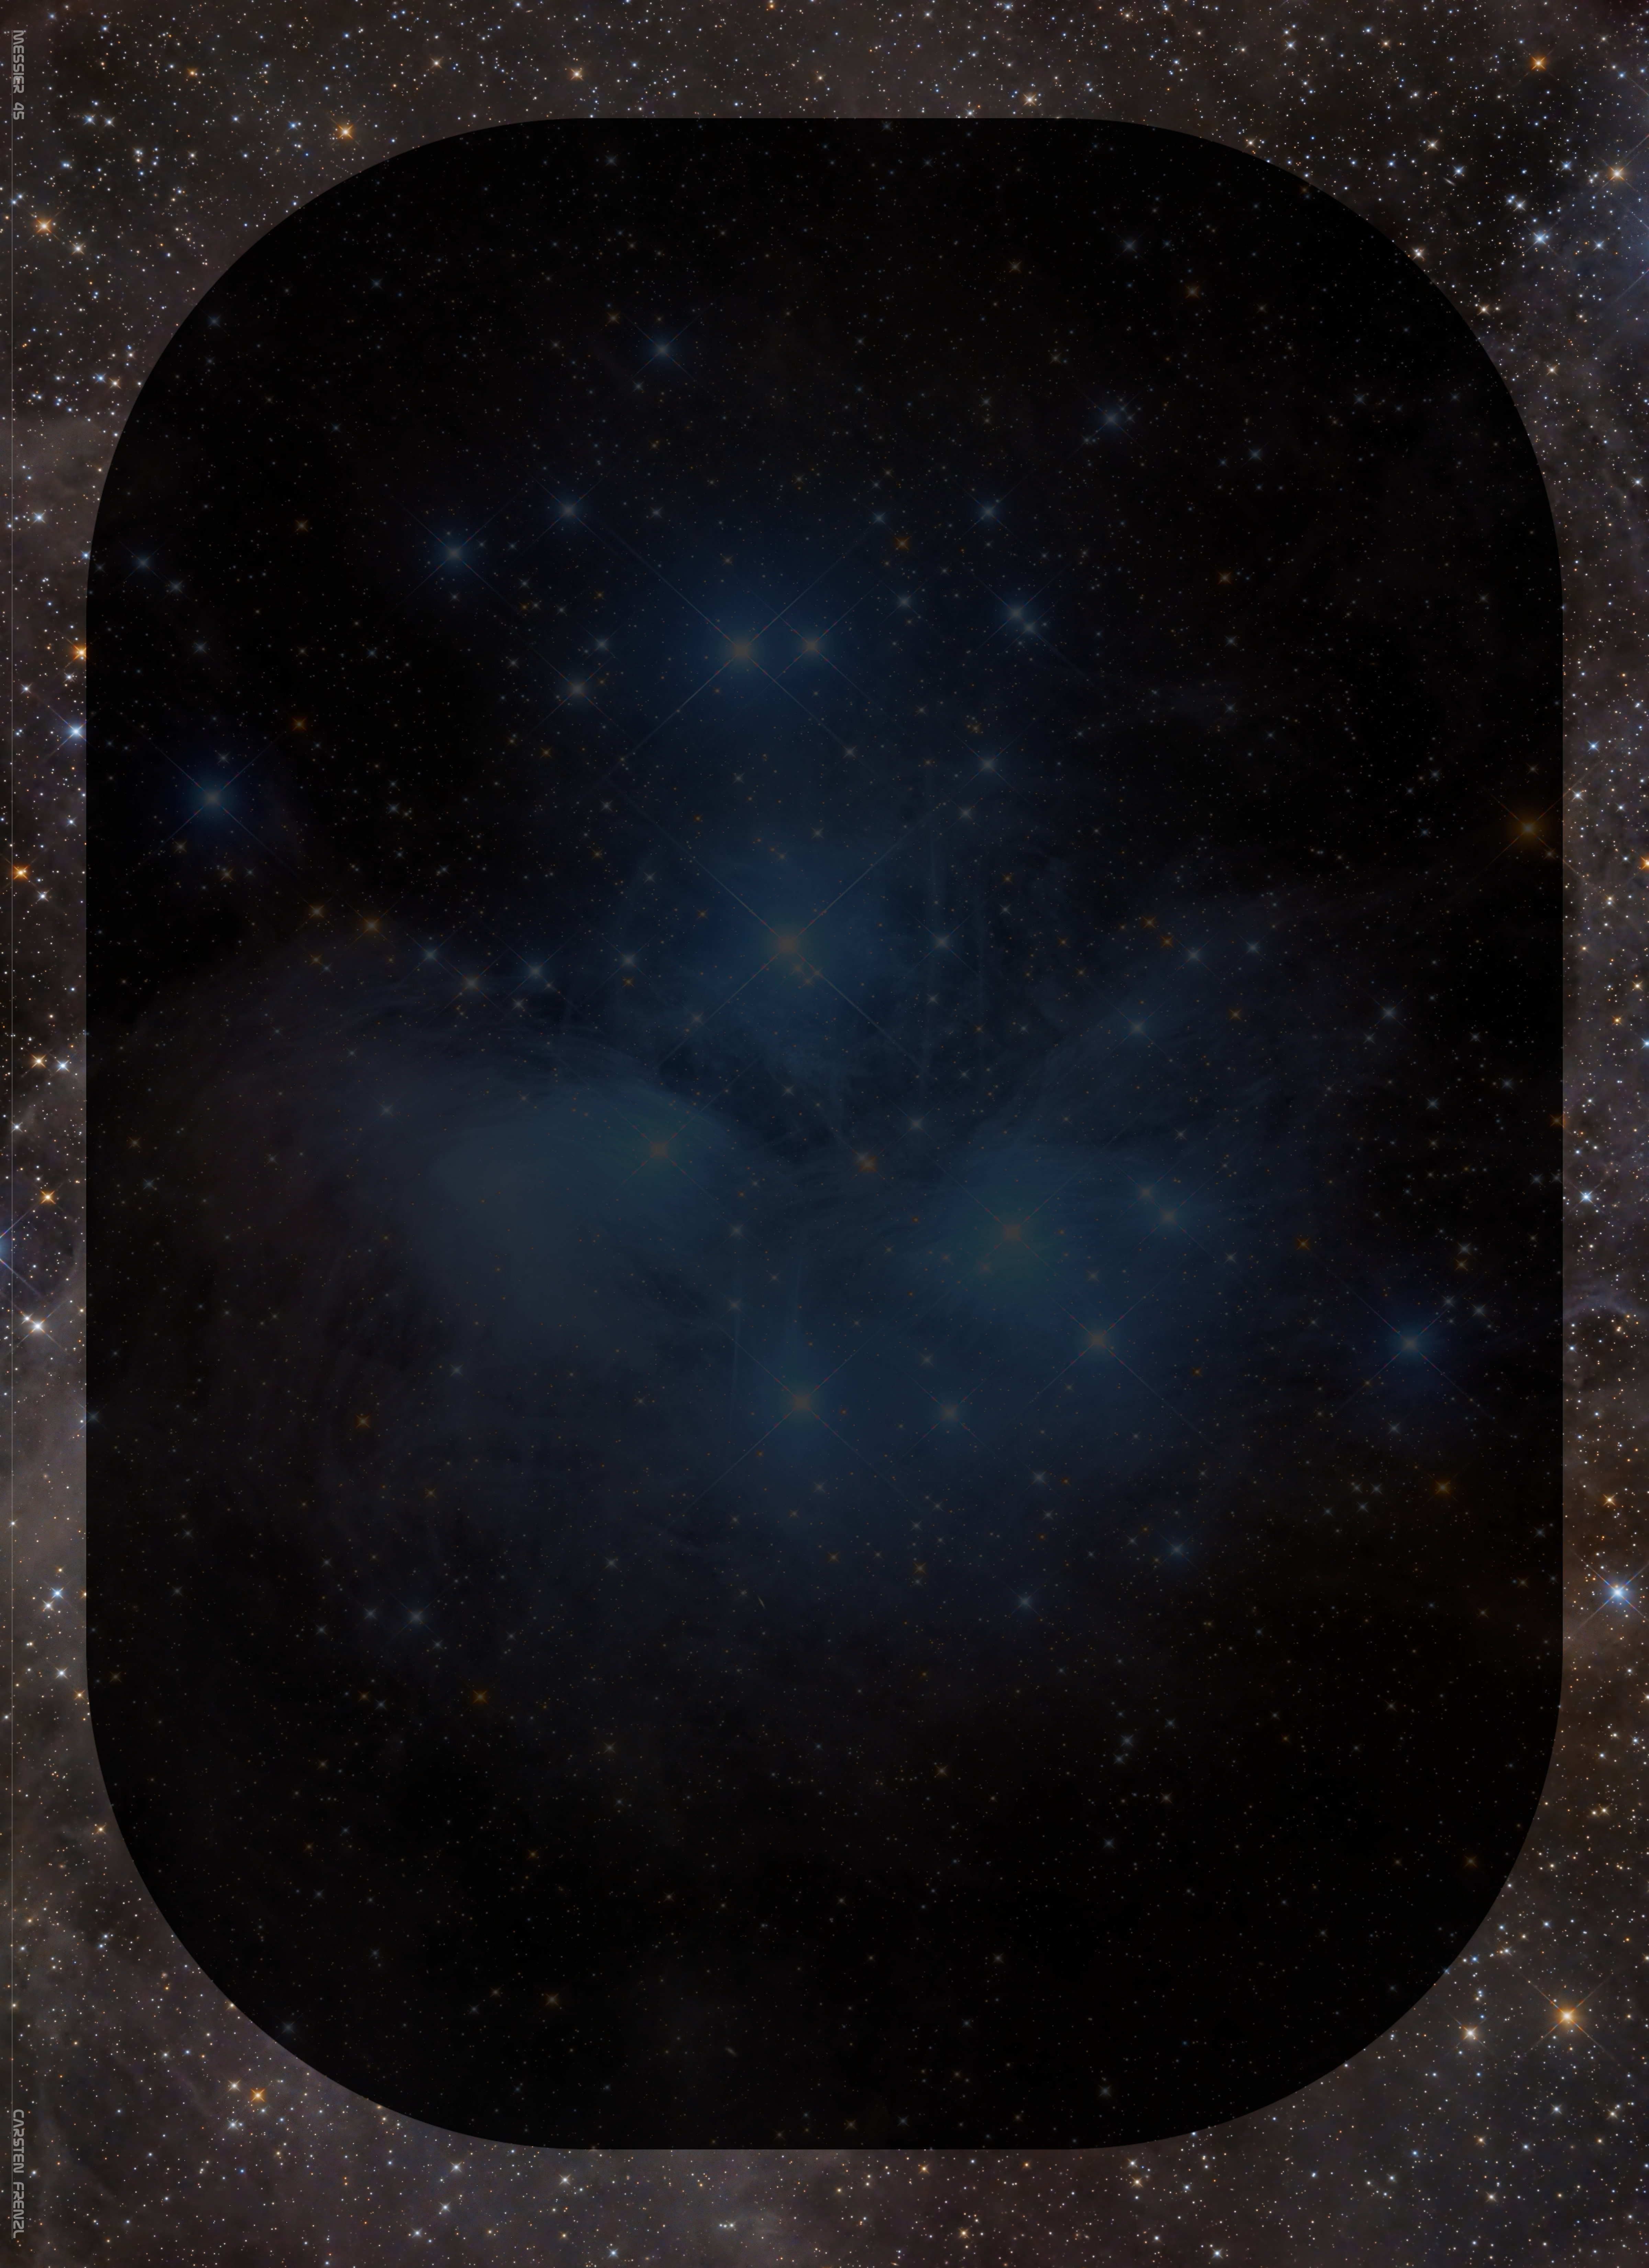
\includegraphics[width=\paperwidth,height=\paperheight]{pleiades.jpeg}}

\renewcommand\thefootnote{{\bfseries\color{SkyBlue}{\arabic{footnote}}}}
\let\oldfootnote\footnote
    \renewcommand{\footnote}[1]{\oldfootnote{{\normalsize\bfseries\color{SkyBlue}#1}}}
\begin{titlepage} % Suppresses headers and footers on the title page
	\centering % Centre everything on the title page
	\scshape % Use small caps for all text on the title page

	%------------------------------------------------
	%	Title
	%------------------------------------------------
	
	\rule{\textwidth}{1.6pt}\vspace*{-\baselineskip}\vspace*{2pt} % Thick horizontal rule
	\rule{\textwidth}{0.4pt} % Thin horizontal rule
	
	\vspace{0.75\baselineskip} % Whitespace above the title

        {\Huge Emanuel Swedenborg \\as a Cosmologist \\} % Title
	
	\vspace{0.75\baselineskip} % Whitespace below the title
	
	\rule{\textwidth}{0.4pt}\vspace*{-\baselineskip}\vspace{3.2pt} % Thin horizontal rule
	\rule{\textwidth}{1.6pt} % Thick horizontal rule
	
	\vspace{1\baselineskip} % Whitespace after the title block
	
	%------------------------------------------------
	%	Subtitle
	%------------------------------------------------
	
	{By \\\Large Svante Arrhenius\\} % Subtitle or further description
	
	\vspace*{1\baselineskip} % Whitespace under the subtitle
	
	%------------------------------------------------
	%	Editor(s)
	%------------------------------------------------

        {\small With four Plates.}
 
        %------------------------------------------------
	%	Cover photo
	%------------------------------------------------
	
	%\includegraphics[scale=1]{cover}
	
	%------------------------------------------------
	%	Publisher
	%------------------------------------------------
		
	\vspace*{\fill}% Whitespace under the publisher logo
	
	% Publication year
	
	{Stockholm, 1908} % Publisher
 
        {\small Aftonbladets Tryckeri}

	\vspace{1\baselineskip} % Whitespace under the publisher logo

        Internet Archive Online Edition  % Publication year
	
	{\small Attribution NonCommercial ShareAlike 4.0 International } % Publisher
\end{titlepage}
\clearpage
\Large
\setlength{\parskip}{1mm plus1mm minus1mm}
\paragraph{}
The\footnote{Translated by Alfred H. Stroh from the original Swedish and revised by the author. Now reprinted from the Introduction to Vol. 2. of the edition of Swedenborg's scientific texts under publication by the Royal Swedish Academy of Sciences at Stockholm: Emanuel Swedenborg, Opera quaedam aut inedita aut obsoleta de rebus naturalibus, nunc edita sub auspiciis Regiae Academiae Scientiarum Suecicae, 2., Cosmologica, introductionem adiunxit Svante Arrhenius, edidit Alfred H. Stroh. Holmiae, ex officina Aftonbladet, 1908. Four plates from Part 3. of Swedenborg's \emph{Principia} of 1734, illustrating his theories of the development of the solar system and of the constitution of matter, are reproduced at the close of this contribution.} present volume of Swedenborg's scientific works contains his perhaps most highly valued work ``Principia rerum naturalium.''\footnote{In 1721 Swedenborg published at Amsterdam a \emph{Prodromus Principiorum rerum naturalium}, reprinted in Vol. 3. of this series. The \emph{Principia rerum naturalium}, printed in the present volume, 1-191, is in all probability the manuscript work referred to by Swedenborg in a letter dated Nov. 27, 1729, printed in Vol. 1. 321. In 1734 Swedenborg published at Dresden and Leipsic three folio volumes entitled \emph{Opera Philosophica et Mineralia}, the first volume being his final \emph{Principia rerum naturalium}. A summary of the final \emph{Principia}, left in manuscript by Swedenborg, is printed in the present volume, 207-262 and also the entire \emph{Third Part} of the \emph{Principia} of 1734. 263-368.} In this work he attempts to give a philosophical presentation of what we might call molecular structure. Now since Swedenborg considered everything in the world, the small as well as the great, to be constructed according to the same fundamental principles, he has also in this work presented his views concerning the structure of the solar and world systems, which views have won considerable praise for the reason that the planets are described as having gone forth from the sun by means of a kind of centrifugal expulsion, a view which subsequently became classical in the works of Buffon, Kant and especially of Laplace. We also find in Swedenborg's \emph{Principia} reflections concerning the relation of the solar system to the milky way which remind us very much of the later expressions of Wright, Kant and Lambert. In this Introduction Swedenborg's cosmology and physics as set forth in the \emph{Principia} will be especially considered, but notes concerning his numerous contributions to physics, and also to chemistry, will be found in Vols. 1. and 3. of this series.

As concerns the printed \emph{Principia}, Swedenborg has divided it into three parts. The contents of the first and third parts are for the most part contained in the hitherto unprinted \emph{Principia}, published below. 1-191. They are mainly of a natural philosophical content, which is also referred to by Swedenborg in the Appendix to the printed \emph{Principia}. 360. On the other hand the second part is of physical content and Swedenborg there renders an account of a great number of experiments with the magnet. In this second part there are also found numerous references to the works of other investigators, while such references are altogether lacking in the first and third parts, which are clearly based exclusively upon the author's philosophical thinking. Of the first and second parts a summary by Swedenborg has been printed, 207-262, corresponding for the most part to the portions italicized by Swedenborg in the printed \emph{Principia}. The third part, which chiefly contains the presentation of Swedenborg's cosmology, has been reprinted unabridged. 263-368. It is also without doubt this part of Swedenborg's scientific writings which more than any other has attracted general attention.

In order to obtain a general view of the contents of this extended work I have made a comparative investigation of the general conceptions in Swedenborg's time concerning matter and especially concerning the cosmological problems, the results of which I here reproduce.

Chemistry in those times occupied a very undeveloped standpoint. The four elements set up by Empedocles still governed the presentation of the chemical phenomena. In physical considerations, however, the conceptions admitted in chemistry were considerably modified. Descartes, who without doubt exercised the greatest influence on Swedenborg's views, supposed that originally there was only one kind of material particles. By their striking each other their corners were knocked off, so that there were formed particles completely round and transparent, which were called ``particles of the second kind.'' Out of the knocked off corners there was formed a fine dust of ``particles of the first kind,'' which formed the fixed stars. They corresponded to the fire or light particles of those times. By their condensation there were formed opaque grosser ``particles of the third kind,'' which occur in the sun spots; and by their further condensation were formed ``particles of the fourth kind,'' which constitute the earth's crust.

It may be seen from this that the conception of Descartes had scarcely anything in common with that which now obtains. No other experience lies at the basis of this supposition than that bodies of very differing physical properties occur. There is no further explanation of the dependence of these physical properties upon the supposed peculiarities of the particles.

In Swedenborg's work no other change is made in these conditions than that the number of particles is increased and an attempt made to derive all of them from the mathematical point.

This section is not of particular interest, but of the greater interest is his treatment of the cosmological problems, which has also attracted considerable attention. We there find expressed various views which correspond more closely to our present conceptions than do those of Swedenborg's predecessors.

In the field of the natural sciences cosmology, or the doctrine of the origin and development of the heavenly bodies, is considered to be a part of astronomy. But on examining this chapter of astronomy it is found that most of the astronomers were not attracted by the cosmological problems, which have been worked upon for the most part by the philosophers. Laplace, whose contribution to our cosmological conception is often brought forward as one of the foremost truths of science, has published it in a short note at the close of his great work \emph{Exposition du système du monde}. On the other hand Kant has treated the same subject at great length in his \emph{Naturgeschichte und Theorie des Himmels}. This peculiarity is easily explained by the fact that while ordinary astronomical work is rather uniform and demands an accuracy exceeding that which is found in the other exact sciences, the cosmological presentations are usually characterized by general features with rather little precision, which are derived from very different branches of science and for the working out of which fancy is used much more than calculation.

It is as a link in the long chain of development of the cosmological conceptions, reaching back all the way to the oldest Greek philosophers, that Swedenborg's cosmological contributions are of considerable interest. Anaximander (611-547 \textsc{bce}) darkly hints that an infinite number of heavenly bodies was formed out of the original chaos by some kind of a circular motion. Empedocles (about 450 \textsc{bce}) also has a very uncertain conception that the heavenly bodies have been separated out from an originally uniform chaos. Similar views are expressed by Anaxagoras, the teacher of Pericles. These first attempts at presenting the evolution of the world were, however, forgotten under the influence of Aristotle's doctrine and the tradition of the church during the middle ages. The man who again took up the old problem was not at all an astronomer like Copernicus or Kepler, but the philosopher Giordano Bruno. He attacked the reigning doctrine in the most violent manner and took the position that the world is infinite and that the fixed stars are suns, around which inhabited planets revolve. He considered the planets to be floating in an infinite, transparent ocean of ether.

To this last doctrine Descartes gave a more scientific formulation. Having observed that all the planets are borne forward around the sun in the same direction, he concluded that this depended upon a vortex formed around the sun by the ocean of ether, which vortex when observed from the sun's north pole flows round from right to left and thus drags along with itself the planets which float in it. The planets he assumed to have entered the vortex from without, from cosmical space, where they once were suns, each surrounded by its own vortex. These suns had however been extinguished and the vortex circling around them weakened, after which they were drawn into a neighboring mighty solar vortex. For our manner of viewing these things this conception that the planets are dragged along by a vortical ocean of ether seems very unjustifiable. But the conditions were altogether different in the time of Descartes. He did not know about Newton's gravitation. If the planets were not dragged along but moved themselves independently, they would travel in straight paths and soon move away from the sun. This ought indeed also to be the case with the particles of the ocean of ether. That they did not move away Descartes could explain in this way only, that they met resistance from other ether particles which were in vortices around neighboring fixed stars and so prevented the parts of the solar vortex from penetrating into foreign regions. It was therefore very natural to assume such a vortex around the sun. Descartes assumed that the vortex existed perpetually.

Swedenborg, although he makes no mention of Descartes in the \emph{Principia}, was without doubt most strongly influenced by the teachings of his great predecessor. The presentation of the system of the world as given by Descartes was presumably referred to in the lectures at Uppsala as a truth generally received, whose author was not especially pointed out since the views displaced by him were not thought worthy of mention. Swedenborg has received from Descartes the doctrine of vortices of ether around the fixed stars. But in this doctrine he has made two modifications. He has assumed that the vortical motion arose gradually and did not exist from the beginning. This view, also held by Kant, may be thought to have a philosophical advantage over that of Descartes, but it is opposed to the fundamental principles of mechanics and is therefore untenable from the standpoint of natural science, wherefore it was also abandoned by Laplace.

The other modification of the views of Descartes has won much more approval. Not without foundation did it seem to Swedenborg simpler to assume that the planets and moons of the solar system proceeded from the solar mass instead of having wandered in from portions of space lying outside of the solar system. This thought has been taken up by Buffon, Kant and Laplace and is the fundamental thought in the admired hypothesis of Laplace. As regards details Swedenborg diverges essentially from his successors. Kant and Laplace assumed that the solar matter was originally spread out over a very wide space, which extended beyond the outmost planets. There, according to Kant, were formed planets by the aggregation of masses of matter; according to Laplace, by separation out of the rotating mass as the result of centrifugal force. Swedenborg on the other hand had assumed that the solar vortex never had so great an extension. The planets had been formed by a centrifugal force depending upon a continually increasing vortical motion of the solar mass, as a result of which its outmost parts were separated and cast out, having drawn themselves together into globes corresponding to the present planets and moons of the planetary system. Afterwards these heavenly bodies had been gradually borne away from the sun to the positions they now occupy. There they are drawn along by the solar vortex like ships by flowing water. A similar view concerning the departure of the planets from the sun was also later expressed by Buffon, but he differs from Swedenborg in this, that Buffon assumed a concussion caused by a comet which by breaking in from outside and striking the sun gave occasion to the casting out of shattered portions of it. In recent times, however, the famous English astronomer G. H. Darwin has expressed a view concerning the removal of the planets from the sun by means of the influence of the tides. This influence acts as a brake upon the central body, by means of which the planet circling around it is lifted from the centre of its path. The rotation energy of the central body is thus changed into potential energy in the planet. Thus the planet's time of revolution is increased. In the same way the moon has been lifted up from its central body the earth, whose speed of rotation has thus been decreased, so that the length of a day has much increased. The tides have therefore had the double influence of lengthening the day as well as the year.

These two statements are found to be already strongly advanced by Swedenborg, although he did not know that the influence of the tides could be adduced as a cause.

Between the times when Descartes and Swedenborg appeared upon the scene falls the period in which Newton made his remarkable discovery of the universal gravitation (1686). This led to the admission that space is empty, since it does not offer any resistance to the movements of the planets and moons. Another consequence was this, that it is now generally supposed that bodies act upon each other at a distance by gravity. This conclusion, however, was something so antagonistic to the conceptions of the time as inherited from the old philosophers, that Newton himself sharply expressed his opposition to it. This no doubt occasioned that Newton's views, notwithstanding their surpassing advantages, were for a long time unable to make themselves valid outside of England, to Voltaire being due the honor of having obtained for them an entrance into France and on the continent as a whole (1730). It is rather likely that also Swedenborg was for the above mentioned reason deterred from employing Newton's law as the basis for his cosmological reflections. This was reserved for the great scientist Buffon (the well-matched rival of Linnaeus).

Kant's attempts, however, made after those of Buffon, show far greater kinship with Swedenborg's. Kant's attempt was finally succeeded by Laplace's celebrated nebular hypothesis, in its turn also suffering from essential defects which later times have attempted to remedy.

There is also another cosmological speculation in Swedenborg's work which is of importance. The Pythagoreans of antiquity taught that the expanse of heaven has a similar extension in all directions and consequently is spherical. The middle point of the sphere is occupied by the central fire, an hypothetical heavenly body, in many respects corresponding to the sun, which also later replaced the central fire as the middle point of the world. Notwithstanding that this view of the sun's central position was the prevailing one, and is for example accepted by Copernicus, there was not lacking even in ancient times another opinion, presumably first expressed by Democritus, the greatest natural philosopher of antiquity, which opinion was this, that the sun is similar in rank to the stars. He also held that the milky way is a collection of sun-resembling stars. Neither did Giordano Bruno consider the sun to be the middle point of the world, but similar in rank to the other stars. This view was also afterwards expressed by Descartes and Swedenborg. Swedenborg added a remarkable expression concerning the system of the milky way, which has afterwards in a somewhat changed form been taken up by a number of authors in the field of cosmology. He had, like Descartes before him, been much occupied by those lines around a magnet called by us lines of force, which he believed depended upon emanations of magnetic matter from the magnet. Such conceptions are already found in Lucretius, who probably borrowed them from Democritus, as also in a highly developed form in Descartes. The lines of force lie most closely together around the axis of the magnet, with which when most nearly adjacent they run parallel. Now Swedenborg supposed that everything in the world is constructed according to a common plan. Therefore the arrangement of the least parts of the magnetic matter should be mirrored in that system of order which ought to prevail between the suns. Now since the suns are seen to be packed most closely along the milky way, it follows that this ought to correspond to an axis in the system of the suns. Swedenborg has not expressed himself concerning the remarkable circumstance that this axis should likely be straight, in which case the milky way ought to look like a semicircle in the sky. But instead this arrangement forms a closed belt around the vault of heaven. One can certainly also suppose magnetic lines of force which form a circle, as for example in a ring-shaped magnet, and we may form a picture of the milky way in this manner, but it would be peculiar if Swedenborg had not mentioned that he had such a thought in case he really did think of this possibility. This explains why Nyrén,\footnote{See \emph{Vierteljahrschrift der Astronomischen Gesellschaft}, 1879. --- The contribution of Professor Nyrén will follow in this series of papers. --- Ed.} who has expressed himself in regard to Swedenborg's view of this matter, considered that it must be supposed that Swedenborg by ``axis'' meant something quite different from other authors, namely, ``aequator.'' If this had been the case, Swedenborg's opinion would have closely agreed with that which was expressed sixteen years later, and probably independently, by the Englishman Wright, who considered the milky way as corresponding to the ecliptic of the system of the suns. Kant was delighted with Wright's thought and took it up, without, however, according to Nyrén's opinion --- Nyrén having had access to the exceedingly rare work of Wright --- having added anything essential to it.

Swedenborg also expressed the opinion that there are still greater systems in which the milky ways are elements, and so forth. This opinion closely agrees with a view, highly valued by many, expressed by Lambert in his ``Kosmologische Briefe,'' of the year 1761.

If we briefly summarize the ideas, which were first given expression to by Swedenborg, and afterwards, although usually in a much modified form --- consciously or unconsciously --- taken up by other authors in cosmology, we find them to be the following:
\begin{itemize}
    \item The planets of our solar system originate from the solar matter --- taken up by Buffon, Kant, Laplace, and others.

    \item The earth --- and the other planets --- have gradually removed themselves from the sun and received a gradually lengthened time of revolution --- a view again expressed by G. H. Darwin.

    \item The earth's time of rotation, that is to say, the day's length, has been gradually increased --- a view again expressed by G. H. Darwin.

    \item The suns are arranged around the milky way --- taken up by Wright, Kant and Lambert.

    \item There are still greater systems, in which the milky ways are arranged --- taken up by Lambert.
\end{itemize}
\paragraph{}
What now is the value of the cosmological principles in general? To this question many very differing answers are given. To indicate this we may refer to the widely differing recognitions of Kant's cosmological work which, have been made in various quarters. Du Bois Reymond says that ``with Kant ends that series of philosophers who were in complete possession of the scientific knowledge of their times and who participated in the work of scientists.'' That this view is untenable, is clear from H. L. Vogel's expressions: ``If one now make allowance for this fundamental error, (that Kant supposed the circling movement of the planetary system not to have existed from the beginning, but to have gradually developed itself), Kant's theory contains so many errors and difficulties in particular points, that it now actually is without any value.'' These difficulties and errors are, however, of such a nature that they should have been apparent even in Kant's time to a man schooled in the laws of mechanics --- as all the essential principles of mechanics were already known at that time.

The great Helmholtz also regards Kant's cosmology as being of high value. He says of it ``that it together with a series of the most happy thoughts sped far ahead of his times.'' It can scarcely be supposed that the acute Helmholtz made so cursory an examination of Kant's ``Naturgeschichte und Theorie des Himmels'' as not to have discovered the grievous errors in the laws of mechanics which are incident to practically every portion of this work. We must therefore suppose that Helmholtz considered Kant's cosmological speculations as having a very high value even although their execution on the mechanical side is untenable. This, namely, is quite supposable, for the cosmological speculations have a philosophical side which is of at least as great significance as their mechanical side. So, for example, we find in the cosmological ideas of Giordano Bruno, which must indeed be described as belonging to the most remarkable in the world's history, no new mechanical considerations at all which are of any value. He has taken up the view of Aristarchus and Copernicus that the earth moves around the sun; he furthermore expresses the grand thought that the earth is but a diminishing little particle in infinite stellar space, since innumerable stars are like our sun surrounded by circling inhabited planets --- already 150 years earlier Nicolaus Cusanus had for the rest expressed the view that other heavenly bodies are inhabited --- and he vehemently rose up in opposition to the prevailing astrological superstition, which lamed scientific investigation, the view, namely, that not only the sun, but also the heavenly bodies, exercise a powerful influence upon events on the earth and especially on men. It is hardly possible to express cosmological opinions of a more deeply reaching significance, and still no principles of mechanical learning enter into them. Bruno also had to pay with his life for his daring defiance of the reigning, and as we now know, altogether false views of the time. He was in truth far ahead of his times.

To those who have valued Kant very highly belong furthermore the ingenious but in high degree eccentric German astrophysicist Zöllner, and in later times Ebert in connection with the edition of Kant's above mentioned work edited by him in Ostwald's ``\emph{Klassiker}.'' Here belong also Haeckel and C. Wolf. For the rest later scientific investigation is rather united in depreciating the value of Kant's work, as for example Düring in his \emph{Kritische Geschichte der Principien der Mechanik} (1873), Count L. Pfeil (1893), Eberhard (Dissertation, Munich, 1893), Gerland (1905), Holzmüller (1906) and Hoppe (1906), and it may be added H. L. Vogel in Newcomb-Engelmann's \emph{Populäre Astronomie} (1905).

All of the above mentioned authors have considered Kant's work from the mechanical standpoint and have not concerned themselves with the great leading ideas in their general scope. On the other hand a philosopher König has in his work ``Kant und die Naturwissenschaft'' (1907) ranked himself on the other side. C. Wolf also emphasizes the thoughtful poesy --- \emph{i. e.}, the philosophical depth --- in Kant's expressions. Haeckel has also without doubt permitted himself to be guided by a philosophical (monistic) manner of treatment in his ``Natürliche Schöpfungsgeschichte.''

It is therefore explained why the cosmological thoughts may be called grand and wonderful, as for example Kant's thoughts in this field, although their execution does not agree with the laws of physics. Not even the great master in the field of celestial mechanics, Laplace, has completely escaped this fate. It is now recognized by all that his so highly praised nebular theory in many points conflicts with the laws of mechanics, although it indeed in that respect is far better than Kant's attempt. And besides it is in conflict with various astronomical and physical discoveries, among which at least one, that of the direction in which the moons of Uranus revolve, was made when he was still in his prime. There is however no one prepared to deny that this cosmological work of Laplace, although it demands working over in almost all details, nevertheless belongs to the most important scientific works which have been executed.

To take another example, one of Kant's predecessors in antiquity, the famous natural philosopher Anaxagoras, taught that the original chaos had been gradually arranged in order, so that the heavenly bodies which now exist were formed, that the sun was an enormous glowing lump of iron and that the other stars were also glowing by their rubbing against the surrounding ether. Most thinkers are no doubt disposed to regard his expression that the sun is made of iron as a worthless curiosity. I however permit myself to entertain an altogether different opinion as to this point. Spectrum analysis has taught us that iron probably constitutes a most essential part of the sun's matter. Observation of the constitution of metallic meteorites teaches us that iron is without comparison the most important metal in them, and from various considerations we view it as probable that the earth's chief mass is iron. Anaxagoras was therefore right, according to all that we know. That he conceived the sun as consisting of iron depended without doubt upon his being led by some circumstance to the important conclusion that iron plays the chief role in inorganic nature. This was a stroke of genius and hardly an accident. In like manner would a superficially judging scientist shrug his shoulders on hearing the naive view that the stars are glowing because they rub against the ether. We know indeed that this does not at all agree with the view of our times. But I maintain nevertheless that under this formally incorrect view is hidden one of the greatest thoughts ever expressed. Scarcely one hundred years ago most astronomers, and among them the leaders, as Herschel and Laplace, had no idea that the sun required any storehouse from which it might draw the enormous quantities of heat which it pours forth, partly in the form of light. They did not reflect concerning this question. On the other hand Kant as a philosopher did this, and also Buffon and many others before him, but among all known philosophers Anaxagoras was probably the first to do so. He could not suppose that the stars ought not to have become extinct long ago on account of loss of heat, had not heat in some way been sustained. The mechanical part of the above mentioned conception of Anaxagoras is untenable, but the idea is nevertheless grand.

Now it is very striking that all those who before Laplace made contributions to the development of the cosmological ideas were natural philosophers, possibly with the exception of Buffon and Descartes who were also scientists of note. But it is no doubt most correct to consider their cosmological works as being for the most part natural philosophy. The same is also true of Swedenborg's work in that he labored but little in working out in physics his widely comprehensive and most remarkable ideas.

A question still remains to be explained, and that is to what extent Swedenborg's ideas have formed the basis of the works of his successors. That one among them who agrees most closely with Swedenborg is Kant, of whom it is well known that he had applied himself to Swedenborg's works. Kant himself says in 1766 that Swedenborg as if by inspiration had discovered scientific relationships which Kant had only been able to explain after many and lengthy investigations. It is for those who compare Kant's speculations concerning inhabited worlds in his above mentioned work with Swedenborg's accounts of his visions quite manifest that Kant has borrowed his ideas from Swedenborg and clothed them in more philosophical garments. It is therefore not improbable that he has also in other parts of the same work been under Swedenborg's immediate influence and worked over his ideas. On the other hand it does not seem as if Wright had known Swedenborg's similar thoughts. I cannot express myself more decidedly since I have not had access to the original, but it would appear as if Nyrén considered Wright's work to be independent of Swedenborg's. As concerns Buffon, it is known that he possessed Swedenborg's \emph{Principia} in 1736 and it is indeed possible that he was led to his cosmological speculations through Swedenborg's work. But Buffon's views differ in high degree from Swedenborg's, so that it would be incorrect to hold that he derived any great service from Swedenborg's opinions. There is indeed no doubt that Buffon knew the vortical theory of Descartes, which was at that time generally promulgated in the universities, which theory Buffon's views resemble as little as they do Swedenborg's. Laplace knew Buffon's views, but hardly Kant's and still less Swedenborg's.

The chief interest in Swedenborg's cosmological conceptions lies in this, that they form a link between the cosmological conceptions of the ancient philosophers and of Descartes on the one side and those of Kant on the other side. Similarly to the conceptions which they connect, Swedenborg's are little developed in the mechanical direction, so that the chief weight must be laid on their natural philosophical part.

That Swedenborg himself considered his \emph{Principia} to be chiefly of philosophical content appears not only from the introduction ``on the means which lead to true philosophy and on the truly philosophical man,'' but also especially from the Appendix, 360, where it is emphasized that his system is built of the concepts ``finita,'' ``activa,'' and ``elementaria.'' He says that he has not published his work to win the favor of the learned world, or a name or fame, neither will it concern him if no one will give recognition to his work --- in this respect he takes an entirely different position about six years before in the hitherto unprinted \emph{Principia}. A man who is striving to find the truth of philosophy does not concern himself as to such things. ``Neither do I wish to ask anyone to depart from the principles of the illustrious and ingenious authors and to accept my own, wherefore I have not wished to refer to the philosophy or name of anyone, in order not to wound anyone or to contradict another's opinion and not to appear to wish to in any wise diminish his renown.'' ``Truth is one and speaks for itself.''

He however refers to a single philosopher, remarkably enough none more significant than Christian Wolff, who ``has contributed much to the extension of true philosophy.'' To him Swedenborg expresses great thankfulness for the use he has had of Wolff's works in the revision of the \emph{Principia}. It has however not been possible for me after comparing it with the works of Wolff referred to, to find those parts of Swedenborg's presentation in which he has permitted himself to be influenced by Wolff's views, excepting in the use of certain terms.

One must admit that it is a grand thought to attempt to furnish an explanation of the world according to which a complete harmony reigns between the greatest and the least --- the stellar system and the atom --- or even according to Swedenborg's conception with its least part, the material point. It can also be easily understood why Swedenborg, who believed that he had happily solved this problem, felt the deepest satisfaction in a work which had occupied so large a portion of his life.
\clearpage
\vspace*{\fill}
\begin{figure}[H]
\centering
\includegraphics[width=0.75\textwidth,keepaspectratio]{skyblue/emanuelswedenborg-table01.png}
\end{figure}
\vspace*{\fill}
\clearpage
\vspace*{\fill}
\begin{figure}[H]
\centering
\includegraphics[width=0.75\textwidth,keepaspectratio]{skyblue/emanuelswedenborg-table02.png}
\end{figure}
\vspace*{\fill}
\clearpage
\vspace*{\fill}
\begin{figure}[H]
\centering
\includegraphics[width=0.75\textwidth,keepaspectratio]{skyblue/emanuelswedenborg-table03.png}
\end{figure}
\vspace*{\fill}
\clearpage
\vspace*{\fill}
\begin{figure}[H]
\centering
\includegraphics[width=0.75\textwidth,keepaspectratio]{skyblue/emanuelswedenborg-table04.png}
\end{figure}
\vspace*{\fill}
\clearpage
\end{document}
